% Options for packages loaded elsewhere
\PassOptionsToPackage{unicode}{hyperref}
\PassOptionsToPackage{hyphens}{url}
%
\documentclass[
]{article}
\usepackage{amsmath,amssymb}
\usepackage{iftex}
\ifPDFTeX
  \usepackage[T1]{fontenc}
  \usepackage[utf8]{inputenc}
  \usepackage{textcomp} % provide euro and other symbols
\else % if luatex or xetex
  \usepackage{unicode-math} % this also loads fontspec
  \defaultfontfeatures{Scale=MatchLowercase}
  \defaultfontfeatures[\rmfamily]{Ligatures=TeX,Scale=1}
\fi
\usepackage{lmodern}
\ifPDFTeX\else
  % xetex/luatex font selection
\fi
% Use upquote if available, for straight quotes in verbatim environments
\IfFileExists{upquote.sty}{\usepackage{upquote}}{}
\IfFileExists{microtype.sty}{% use microtype if available
  \usepackage[]{microtype}
  \UseMicrotypeSet[protrusion]{basicmath} % disable protrusion for tt fonts
}{}
\makeatletter
\@ifundefined{KOMAClassName}{% if non-KOMA class
  \IfFileExists{parskip.sty}{%
    \usepackage{parskip}
  }{% else
    \setlength{\parindent}{0pt}
    \setlength{\parskip}{6pt plus 2pt minus 1pt}}
}{% if KOMA class
  \KOMAoptions{parskip=half}}
\makeatother
\usepackage{xcolor}
\usepackage[margin=1in]{geometry}
\usepackage{color}
\usepackage{fancyvrb}
\newcommand{\VerbBar}{|}
\newcommand{\VERB}{\Verb[commandchars=\\\{\}]}
\DefineVerbatimEnvironment{Highlighting}{Verbatim}{commandchars=\\\{\}}
% Add ',fontsize=\small' for more characters per line
\usepackage{framed}
\definecolor{shadecolor}{RGB}{248,248,248}
\newenvironment{Shaded}{\begin{snugshade}}{\end{snugshade}}
\newcommand{\AlertTok}[1]{\textcolor[rgb]{0.94,0.16,0.16}{#1}}
\newcommand{\AnnotationTok}[1]{\textcolor[rgb]{0.56,0.35,0.01}{\textbf{\textit{#1}}}}
\newcommand{\AttributeTok}[1]{\textcolor[rgb]{0.13,0.29,0.53}{#1}}
\newcommand{\BaseNTok}[1]{\textcolor[rgb]{0.00,0.00,0.81}{#1}}
\newcommand{\BuiltInTok}[1]{#1}
\newcommand{\CharTok}[1]{\textcolor[rgb]{0.31,0.60,0.02}{#1}}
\newcommand{\CommentTok}[1]{\textcolor[rgb]{0.56,0.35,0.01}{\textit{#1}}}
\newcommand{\CommentVarTok}[1]{\textcolor[rgb]{0.56,0.35,0.01}{\textbf{\textit{#1}}}}
\newcommand{\ConstantTok}[1]{\textcolor[rgb]{0.56,0.35,0.01}{#1}}
\newcommand{\ControlFlowTok}[1]{\textcolor[rgb]{0.13,0.29,0.53}{\textbf{#1}}}
\newcommand{\DataTypeTok}[1]{\textcolor[rgb]{0.13,0.29,0.53}{#1}}
\newcommand{\DecValTok}[1]{\textcolor[rgb]{0.00,0.00,0.81}{#1}}
\newcommand{\DocumentationTok}[1]{\textcolor[rgb]{0.56,0.35,0.01}{\textbf{\textit{#1}}}}
\newcommand{\ErrorTok}[1]{\textcolor[rgb]{0.64,0.00,0.00}{\textbf{#1}}}
\newcommand{\ExtensionTok}[1]{#1}
\newcommand{\FloatTok}[1]{\textcolor[rgb]{0.00,0.00,0.81}{#1}}
\newcommand{\FunctionTok}[1]{\textcolor[rgb]{0.13,0.29,0.53}{\textbf{#1}}}
\newcommand{\ImportTok}[1]{#1}
\newcommand{\InformationTok}[1]{\textcolor[rgb]{0.56,0.35,0.01}{\textbf{\textit{#1}}}}
\newcommand{\KeywordTok}[1]{\textcolor[rgb]{0.13,0.29,0.53}{\textbf{#1}}}
\newcommand{\NormalTok}[1]{#1}
\newcommand{\OperatorTok}[1]{\textcolor[rgb]{0.81,0.36,0.00}{\textbf{#1}}}
\newcommand{\OtherTok}[1]{\textcolor[rgb]{0.56,0.35,0.01}{#1}}
\newcommand{\PreprocessorTok}[1]{\textcolor[rgb]{0.56,0.35,0.01}{\textit{#1}}}
\newcommand{\RegionMarkerTok}[1]{#1}
\newcommand{\SpecialCharTok}[1]{\textcolor[rgb]{0.81,0.36,0.00}{\textbf{#1}}}
\newcommand{\SpecialStringTok}[1]{\textcolor[rgb]{0.31,0.60,0.02}{#1}}
\newcommand{\StringTok}[1]{\textcolor[rgb]{0.31,0.60,0.02}{#1}}
\newcommand{\VariableTok}[1]{\textcolor[rgb]{0.00,0.00,0.00}{#1}}
\newcommand{\VerbatimStringTok}[1]{\textcolor[rgb]{0.31,0.60,0.02}{#1}}
\newcommand{\WarningTok}[1]{\textcolor[rgb]{0.56,0.35,0.01}{\textbf{\textit{#1}}}}
\usepackage{longtable,booktabs,array}
\usepackage{calc} % for calculating minipage widths
% Correct order of tables after \paragraph or \subparagraph
\usepackage{etoolbox}
\makeatletter
\patchcmd\longtable{\par}{\if@noskipsec\mbox{}\fi\par}{}{}
\makeatother
% Allow footnotes in longtable head/foot
\IfFileExists{footnotehyper.sty}{\usepackage{footnotehyper}}{\usepackage{footnote}}
\makesavenoteenv{longtable}
\usepackage{graphicx}
\makeatletter
\def\maxwidth{\ifdim\Gin@nat@width>\linewidth\linewidth\else\Gin@nat@width\fi}
\def\maxheight{\ifdim\Gin@nat@height>\textheight\textheight\else\Gin@nat@height\fi}
\makeatother
% Scale images if necessary, so that they will not overflow the page
% margins by default, and it is still possible to overwrite the defaults
% using explicit options in \includegraphics[width, height, ...]{}
\setkeys{Gin}{width=\maxwidth,height=\maxheight,keepaspectratio}
% Set default figure placement to htbp
\makeatletter
\def\fps@figure{htbp}
\makeatother
\setlength{\emergencystretch}{3em} % prevent overfull lines
\providecommand{\tightlist}{%
  \setlength{\itemsep}{0pt}\setlength{\parskip}{0pt}}
\setcounter{secnumdepth}{-\maxdimen} % remove section numbering
\ifLuaTeX
  \usepackage{selnolig}  % disable illegal ligatures
\fi
\usepackage{bookmark}
\IfFileExists{xurl.sty}{\usepackage{xurl}}{} % add URL line breaks if available
\urlstyle{same}
\hypersetup{
  pdftitle={APUNTS},
  pdfauthor={Ànnia},
  hidelinks,
  pdfcreator={LaTeX via pandoc}}

\title{APUNTS}
\author{Ànnia}
\date{2024-11-19}

\begin{document}
\maketitle

\section{CONFIGURAR L'ESPAI DE
TREBALL}\label{configurar-lespai-de-treball}

Al final del vídeo 1 explica com linkar el repositori de github i el
projecte R. Primer hem descarregat des de la pàgina de GEO el dataset
que volien i a més hem carregat les dades de github per tenir-les a
l'entorn. Per descarregar el dataset ho hem fet des de:
\url{https://www.ncbi.nlm.nih.gov/geo/query/acc.cgi?acc=GSE27174} el
fitxer GSE27174\_RAW.tar. Per simplement carregar les dades de github, a
la terminal he escrit: git clone
\url{https://github.com/ASPteaching/Analisis_de_datos_omicos-Ejemplo_1-Microarrays.git}

\begin{figure}
\centering
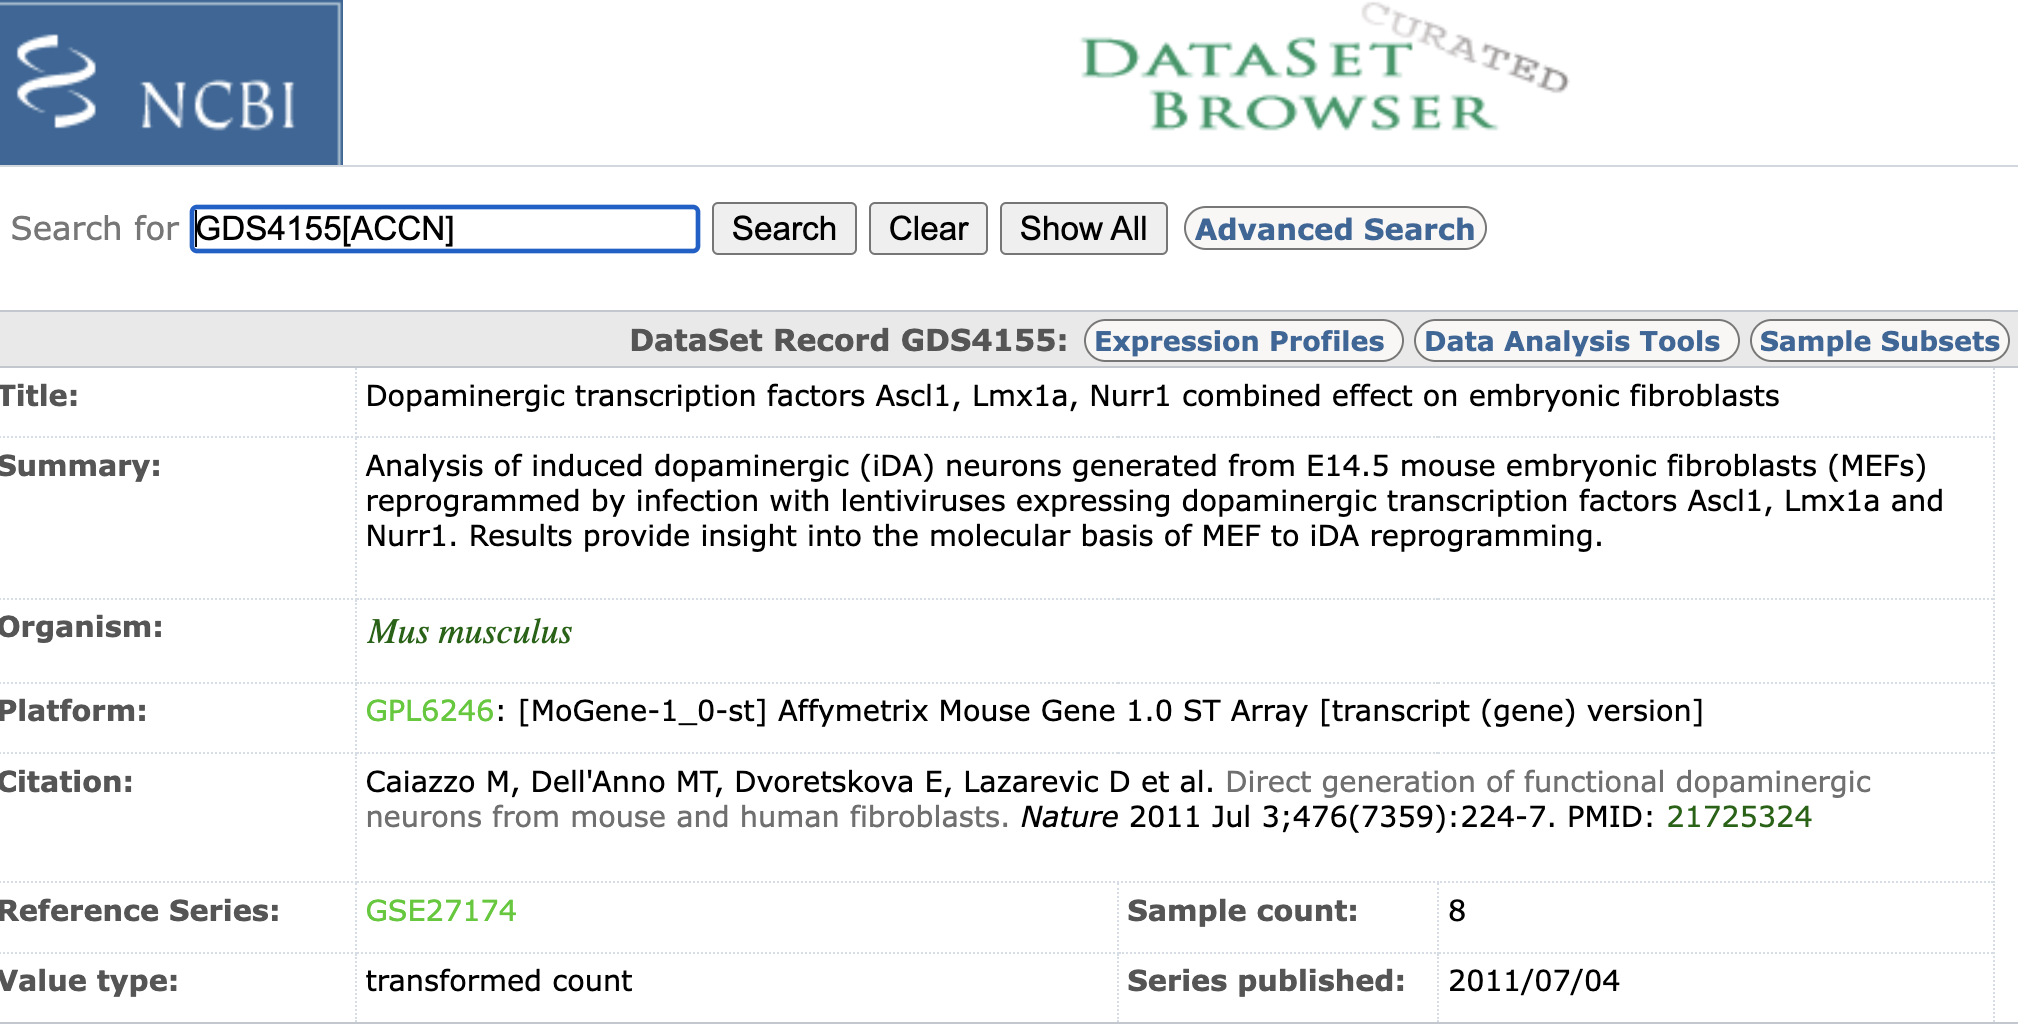
\includegraphics{images/clipboard-1792697817.png}
\caption{WEB GEO}
\end{figure}

A més, hem configurat les dreceres de treball:

\begin{Shaded}
\begin{Highlighting}[]
\FunctionTok{setwd}\NormalTok{(}\StringTok{"/Users/annia/Desktop/UOC/DADES ÒMIQUES/ACT2.2/Series GSE27174"}\NormalTok{)}
\NormalTok{WorkingDir }\OtherTok{\textless{}{-}} \FunctionTok{getwd}\NormalTok{()}
\NormalTok{DataDir }\OtherTok{\textless{}{-}} \FunctionTok{file.path}\NormalTok{(WorkingDir, }\StringTok{"dades"}\NormalTok{)}
\NormalTok{ResultsDir }\OtherTok{\textless{}{-}} \FunctionTok{file.path}\NormalTok{(WorkingDir, }\StringTok{"resultats"}\NormalTok{)}
\end{Highlighting}
\end{Shaded}

Hem creat les dreceres de dades i treball.

\section{CARREGUEM LES DADES I LES
ORGANITZEM}\label{carreguem-les-dades-i-les-organitzem}

Creen un excel format csv on han posat els noms dels datasets
descarregats, si són cas o control, un color segons si són cas o control
i finalment un short name. Una vegada creat, l'importem:

\begin{figure}
\centering
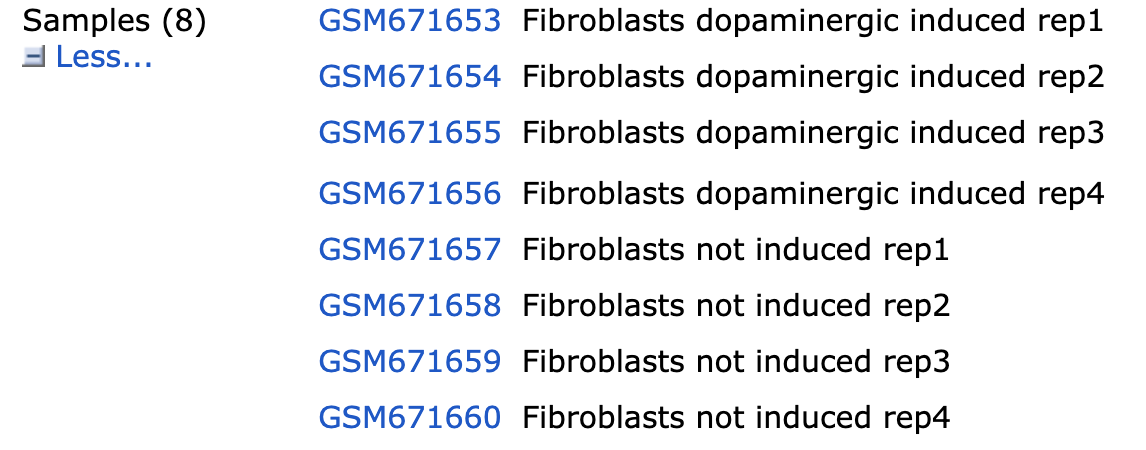
\includegraphics{images/clipboard-1879416855.png}
\caption{Info per passar a csv}
\end{figure}

\begin{Shaded}
\begin{Highlighting}[]
\FunctionTok{library}\NormalTok{(readr)}
\NormalTok{targets }\OtherTok{\textless{}{-}} \FunctionTok{read\_delim}\NormalTok{(}\StringTok{"dades/targets.csv"}\NormalTok{, }\AttributeTok{delim =} \StringTok{";"}\NormalTok{, }\AttributeTok{escape\_double =} \ConstantTok{FALSE}\NormalTok{, }\AttributeTok{trim\_ws =} \ConstantTok{TRUE}\NormalTok{)}
\FunctionTok{View}\NormalTok{(targets)}
\end{Highlighting}
\end{Shaded}

Per tant ja tenim els arxius cel i targets.csv. Ara farem el codi
d'ànalisi. Carreguem tots els paquets que ens ha dit:

\begin{Shaded}
\begin{Highlighting}[]
\ControlFlowTok{if}\NormalTok{ (}\SpecialCharTok{!}\FunctionTok{require}\NormalTok{(BiocManager)) }\FunctionTok{install.packages}\NormalTok{(}\StringTok{"BiocManager"}\NormalTok{)}
\NormalTok{installifnot }\OtherTok{\textless{}{-}} \ControlFlowTok{function}\NormalTok{(pkg) \{}
    \ControlFlowTok{if}\NormalTok{ (}\SpecialCharTok{!}\FunctionTok{require}\NormalTok{(pkg, }\AttributeTok{character.only =}\NormalTok{ T)) \{}
\NormalTok{        BiocManager}\SpecialCharTok{::}\FunctionTok{install}\NormalTok{(pkg)}
\NormalTok{    \}}
\NormalTok{\}}
\CommentTok{\# BiocManager::install() \# Actualiza paquetes instalados}
\NormalTok{BiocManager}\SpecialCharTok{::}\FunctionTok{install}\NormalTok{(}\StringTok{"arrayQualityMetrics"}\NormalTok{)}
\FunctionTok{library}\NormalTok{(arrayQualityMetrics)}
\FunctionTok{installifnot}\NormalTok{(}\StringTok{"pd.mogene.1.0.st.v1"}\NormalTok{)}
\FunctionTok{installifnot}\NormalTok{(}\StringTok{"mogene10sttranscriptcluster.db"}\NormalTok{)}
\FunctionTok{installifnot}\NormalTok{(}\StringTok{"oligo"}\NormalTok{)}
\FunctionTok{installifnot}\NormalTok{(}\StringTok{"limma"}\NormalTok{)}
\FunctionTok{installifnot}\NormalTok{(}\StringTok{"Biobase"}\NormalTok{)}
\FunctionTok{installifnot}\NormalTok{(}\StringTok{"arrayQualityMetrics"}\NormalTok{)}
\FunctionTok{installifnot}\NormalTok{(}\StringTok{"genefilter"}\NormalTok{)}
\FunctionTok{installifnot}\NormalTok{(}\StringTok{"annotate"}\NormalTok{)}
\FunctionTok{installifnot}\NormalTok{(}\StringTok{"xtable"}\NormalTok{)}
\FunctionTok{installifnot}\NormalTok{(}\StringTok{"gplots"}\NormalTok{)}
\FunctionTok{installifnot}\NormalTok{(}\StringTok{"GOstats"}\NormalTok{)}
\end{Highlighting}
\end{Shaded}

Ara crea l'AnnotatedDataFrame:

\begin{Shaded}
\begin{Highlighting}[]
\FunctionTok{library}\NormalTok{(Biobase)  }\CommentTok{\#carreguem biobase}
\NormalTok{targetsDF }\OtherTok{\textless{}{-}} \FunctionTok{read.csv}\NormalTok{(}\AttributeTok{file =} \FunctionTok{file.path}\NormalTok{(DataDir, }\StringTok{"targets.csv"}\NormalTok{), }\AttributeTok{header =} \ConstantTok{TRUE}\NormalTok{, }\AttributeTok{sep =} \StringTok{";"}\NormalTok{)  }\CommentTok{\#llegim el fitxer targets}
\CommentTok{\# ara ja deixa preparats UNS ÍTEMS per després poder generar plots i etc}
\NormalTok{sampleNames }\OtherTok{\textless{}{-}} \FunctionTok{as.character}\NormalTok{(targetsDF}\SpecialCharTok{$}\NormalTok{ShortName)}
\NormalTok{sampleColor }\OtherTok{\textless{}{-}} \FunctionTok{as.character}\NormalTok{(targetsDF}\SpecialCharTok{$}\NormalTok{Colors)}
\CommentTok{\# Crea un objecte AnnotatedDataFrame}
\NormalTok{targets }\OtherTok{\textless{}{-}} \FunctionTok{AnnotatedDataFrame}\NormalTok{(targetsDF)}
\end{Highlighting}
\end{Shaded}

\begin{longtable}[]{@{}
  >{\raggedright\arraybackslash}p{(\columnwidth - 2\tabcolsep) * \real{0.2596}}
  >{\raggedright\arraybackslash}p{(\columnwidth - 2\tabcolsep) * \real{0.7404}}@{}}
\toprule\noalign{}
\begin{minipage}[b]{\linewidth}\raggedright
Annotated Data Frame
\end{minipage} & \begin{minipage}[b]{\linewidth}\raggedright
Expression Set
\end{minipage} \\
\midrule\noalign{}
\endhead
\bottomrule\noalign{}
\endlastfoot
Emmagatzema metadades sobre les mostres en un experiment.

Conté informació com ara el grup experimental, el sexe, l'edat, etc., de
cada mostra.

S'utilitza per organitzar i descriure les mostres en un estudi.

Resum: \texttt{AnnotatedDataFrame}: Metadades de les mostres o dels
gens. & És una estructura més complexa que combina dades d'expressió
gènica amb metadades de les mostres i dels gens.

Conté la matriu d'expressió gènica (on les files són gens i les columnes
són mostres), un \texttt{AnnotatedDataFrame} per a les metadades de les
mostres i un altre \texttt{AnnotatedDataFrame} per a les metadades dels
gens (com ara anotacions de funcions o vies).

És la estructura principal per emmagatzemar i analitzar dades
d'expressió gènica en Bioconductor.

Resum: \texttt{ExpressionSet}: Combina dades d'expressió, metadades de
mostres i metadades de gens. \\
\end{longtable}

Ara el que farem és llegir els arxius CEL i complementar la informació
que tenim:

\begin{Shaded}
\begin{Highlighting}[]
\NormalTok{CELfiles }\OtherTok{\textless{}{-}}\NormalTok{ targetsDF}\SpecialCharTok{$}\NormalTok{fileName  }\CommentTok{\#agafem els noms dels arxius CEL}
\NormalTok{rawData }\OtherTok{\textless{}{-}} \FunctionTok{read.celfiles}\NormalTok{(}\FunctionTok{file.path}\NormalTok{(DataDir, CELfiles), }\AttributeTok{phenoData =}\NormalTok{ targets)}
\end{Highlighting}
\end{Shaded}

\begin{verbatim}
Reading in : /Users/annia/Desktop/UOC/DADES ÒMIQUES/ACT2.2/Series GSE27174/dades/GSM671653.CEL
Reading in : /Users/annia/Desktop/UOC/DADES ÒMIQUES/ACT2.2/Series GSE27174/dades/GSM671654.CEL
Reading in : /Users/annia/Desktop/UOC/DADES ÒMIQUES/ACT2.2/Series GSE27174/dades/GSM671655.CEL
Reading in : /Users/annia/Desktop/UOC/DADES ÒMIQUES/ACT2.2/Series GSE27174/dades/GSM671656.CEL
Reading in : /Users/annia/Desktop/UOC/DADES ÒMIQUES/ACT2.2/Series GSE27174/dades/GSM671657.CEL
Reading in : /Users/annia/Desktop/UOC/DADES ÒMIQUES/ACT2.2/Series GSE27174/dades/GSM671658.CEL
Reading in : /Users/annia/Desktop/UOC/DADES ÒMIQUES/ACT2.2/Series GSE27174/dades/GSM671659.CEL
Reading in : /Users/annia/Desktop/UOC/DADES ÒMIQUES/ACT2.2/Series GSE27174/dades/GSM671660.CEL
\end{verbatim}

\begin{Shaded}
\begin{Highlighting}[]
\CommentTok{\# fa servir la funció read.celfiles i els combina en un objecte.}
\CommentTok{\# file.path(dataDir, CELfiles) construeix un ruta completa pels arxius CEL, que}
\CommentTok{\# genera una ruta per a cada un. phenoData=targets{-}{-}\textgreater{}es fa servir aquest}
\CommentTok{\# objecte com la info fenotípica (metadades de les mostres) associades a les}
\CommentTok{\# dades d\textquotesingle{}expressió}
\NormalTok{rawData}
\end{Highlighting}
\end{Shaded}

\begin{verbatim}
GeneFeatureSet (storageMode: lockedEnvironment)
assayData: 1102500 features, 8 samples 
  element names: exprs 
protocolData
  rowNames: 1 2 ... 8 (8 total)
  varLabels: exprs dates
  varMetadata: labelDescription channel
phenoData
  rowNames: 1 2 ... 8 (8 total)
  varLabels: fileName grupos ShortName Colors
  varMetadata: labelDescription channel
featureData: none
experimentData: use 'experimentData(object)'
Annotation: pd.mogene.1.0.st.v1 
\end{verbatim}

\begin{Shaded}
\begin{Highlighting}[]
\FunctionTok{exprs}\NormalTok{(rawData)  }\CommentTok{\#cada fila representa un gen/sonda del microarray i cada columna és una mostra. Els valors són els nivells d\textquotesingle{}expressió de cada gen.}
\end{Highlighting}
\end{Shaded}

\begin{verbatim}
            1     2     3     4     5     6     7     8
1        5804  4154 10979  6825  6780  7335 10652  5293
2          74    70   156   100   105    94   201    79
3        5691  4192 10243  7134  6666  6819 10532  5183
4          65    73    92   154   134    82    92    70
5          45    44   143    52    58    51   228   113
6          71    86    68    51    86    78   114    54
7        6977  5210 10943  7491  8056  7430 11541  5794
8          84    62   138    66   144    77   143    78
9        6412  4965 11722  7154  7690  7554 11419  5885
 [ reached getOption("max.print") -- omitted 1102491 rows ]
\end{verbatim}

\section{EXPLORACIÓ I CONTROL DE
QUALITAT}\label{exploraciuxf3-i-control-de-qualitat}

Anem a fer un boxplot, que en aquest cas admet un objecte tipus rawData.
Aquest ens ensenyarà la distribució dels valors.

\begin{Shaded}
\begin{Highlighting}[]
\CommentTok{\# BOXPLOT}
\FunctionTok{boxplot}\NormalTok{(rawData, }\AttributeTok{which =} \StringTok{"all"}\NormalTok{, }\AttributeTok{las =} \DecValTok{2}\NormalTok{, }\AttributeTok{main =} \StringTok{"Intensity distribution of RAW data"}\NormalTok{,}
    \AttributeTok{cex.axis =} \FloatTok{0.6}\NormalTok{, }\AttributeTok{col =}\NormalTok{ sampleColor, }\AttributeTok{names =}\NormalTok{ sampleNames)}
\end{Highlighting}
\end{Shaded}

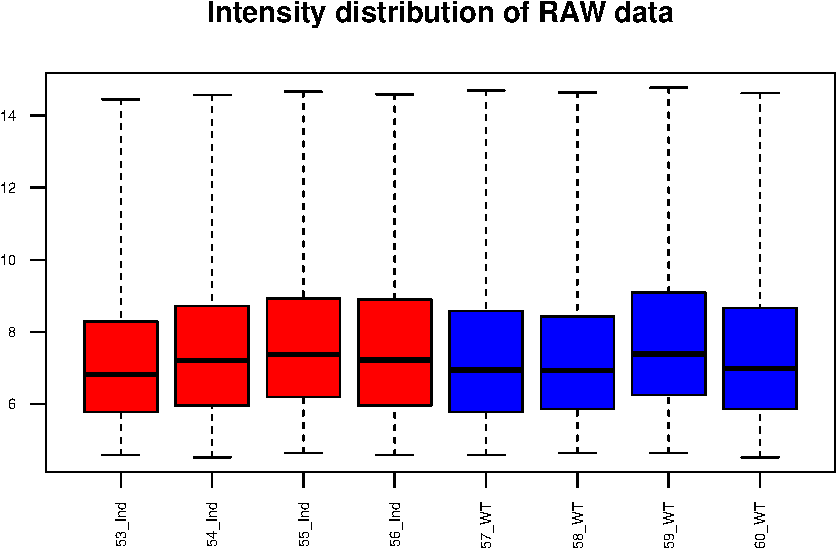
\includegraphics{APUNTS_files/figure-latex/graficosCalidad-1.pdf}

El professor diu que s'han de normalitzar però que no es veuen masses
diferències i que són resultats congruents.

Tot seguit fa un clustering jeràrquic, que ens dóna un tipus
d'informació una mica diferent:

\begin{Shaded}
\begin{Highlighting}[]
\CommentTok{\# HIERARQUICAL CLUSTERING}
\NormalTok{clust.euclid.average }\OtherTok{\textless{}{-}} \FunctionTok{hclust}\NormalTok{(}\FunctionTok{dist}\NormalTok{(}\FunctionTok{t}\NormalTok{(}\FunctionTok{exprs}\NormalTok{(rawData))), }\AttributeTok{method =} \StringTok{"average"}\NormalTok{)}
\FunctionTok{plot}\NormalTok{(clust.euclid.average, }\AttributeTok{labels =}\NormalTok{ sampleNames, }\AttributeTok{main =} \StringTok{"Hierarchical clustering of RawData"}\NormalTok{,}
    \AttributeTok{cex =} \FloatTok{0.7}\NormalTok{, }\AttributeTok{hang =} \SpecialCharTok{{-}}\DecValTok{1}\NormalTok{)}
\end{Highlighting}
\end{Shaded}

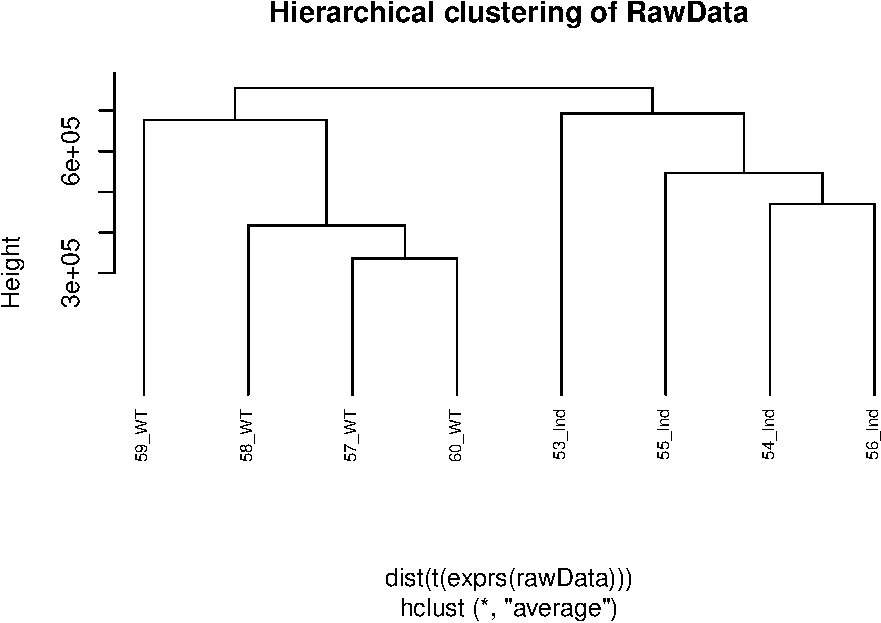
\includegraphics{APUNTS_files/figure-latex/graficosCalidad2-1.pdf}

Ens ensenya com s'agrupen les mostres: veiem que les mostres induïdes
s'assemblen més entre elles i el mateix amb les no induïdes.

Ara farem un PCA: reducció de la dimensionalitat. Ens crea unes
dimensions independents entre sí i cada dimensió explica un \% de
variabilitat. Recordem que a columnes tenim mostres i a files cada gen.
El codi que fan servir és el següent:

\begin{Shaded}
\begin{Highlighting}[]
\CommentTok{\#PRINCIPAL COMPONENT ANALYSIS}
\NormalTok{plotPCA }\OtherTok{\textless{}{-}} \ControlFlowTok{function}\NormalTok{ ( X, }\AttributeTok{labels=}\ConstantTok{NULL}\NormalTok{, }\AttributeTok{colors=}\ConstantTok{NULL}\NormalTok{, }\AttributeTok{dataDesc=}\StringTok{""}\NormalTok{, }\AttributeTok{scale=}\ConstantTok{FALSE}\NormalTok{, }\AttributeTok{formapunts=}\ConstantTok{NULL}\NormalTok{, }\AttributeTok{myCex=}\FloatTok{0.8}\NormalTok{,...) }\CommentTok{\#ha definit una funció per fer el PCA. X serà la matriu d\textquotesingle{}expressió gènica. NO LES ESCALA.}
\NormalTok{\{}
\NormalTok{  pcX}\OtherTok{\textless{}{-}}\FunctionTok{prcomp}\NormalTok{(}\FunctionTok{t}\NormalTok{(X), }\AttributeTok{scale=}\NormalTok{scale) }\CommentTok{\#fa la transposada; escalarà les dades si a l\textquotesingle{}anterior posa TRUE; sinó no.}
\NormalTok{  loads}\OtherTok{\textless{}{-}} \FunctionTok{round}\NormalTok{(pcX}\SpecialCharTok{$}\NormalTok{sdev}\SpecialCharTok{\^{}}\DecValTok{2}\SpecialCharTok{/}\FunctionTok{sum}\NormalTok{(pcX}\SpecialCharTok{$}\NormalTok{sdev}\SpecialCharTok{\^{}}\DecValTok{2}\NormalTok{)}\SpecialCharTok{*}\DecValTok{100}\NormalTok{,}\DecValTok{1}\NormalTok{) }\CommentTok{\#calcula la variància explicada per cada component. }
  \CommentTok{\#print(loads)}
\NormalTok{  xlab}\OtherTok{\textless{}{-}}\FunctionTok{c}\NormalTok{(}\FunctionTok{paste}\NormalTok{(}\StringTok{"PC1"}\NormalTok{,loads[}\DecValTok{1}\NormalTok{],}\StringTok{"\%"}\NormalTok{)) }\CommentTok{\#etiquetes pels eixos amb els \% de cada component}
\NormalTok{  ylab}\OtherTok{\textless{}{-}}\FunctionTok{c}\NormalTok{(}\FunctionTok{paste}\NormalTok{(}\StringTok{"PC2"}\NormalTok{,loads[}\DecValTok{2}\NormalTok{],}\StringTok{"\%"}\NormalTok{))}
  \ControlFlowTok{if}\NormalTok{ (}\FunctionTok{is.null}\NormalTok{(colors)) colors}\OtherTok{=}\DecValTok{1} \CommentTok{\#negre si no s\textquotesingle{}especifica}
  \FunctionTok{plot}\NormalTok{(pcX}\SpecialCharTok{$}\NormalTok{x[,}\DecValTok{1}\SpecialCharTok{:}\DecValTok{2}\NormalTok{],}\AttributeTok{xlab=}\NormalTok{xlab,}\AttributeTok{ylab=}\NormalTok{ylab, }\AttributeTok{col=}\NormalTok{colors, }\AttributeTok{pch=}\NormalTok{formapunts, }
       \AttributeTok{xlim=}\FunctionTok{c}\NormalTok{(}\FunctionTok{min}\NormalTok{(pcX}\SpecialCharTok{$}\NormalTok{x[,}\DecValTok{1}\NormalTok{])}\SpecialCharTok{{-}}\DecValTok{100000}\NormalTok{, }\FunctionTok{max}\NormalTok{(pcX}\SpecialCharTok{$}\NormalTok{x[,}\DecValTok{1}\NormalTok{])}\SpecialCharTok{+}\DecValTok{100000}\NormalTok{),}\AttributeTok{ylim=}\FunctionTok{c}\NormalTok{(}\FunctionTok{min}\NormalTok{(pcX}\SpecialCharTok{$}\NormalTok{x[,}\DecValTok{2}\NormalTok{])}\SpecialCharTok{{-}}\DecValTok{100000}\NormalTok{, }\FunctionTok{max}\NormalTok{(pcX}\SpecialCharTok{$}\NormalTok{x[,}\DecValTok{2}\NormalTok{])}\SpecialCharTok{+}\DecValTok{100000}\NormalTok{))}
  \FunctionTok{text}\NormalTok{(pcX}\SpecialCharTok{$}\NormalTok{x[,}\DecValTok{1}\NormalTok{],pcX}\SpecialCharTok{$}\NormalTok{x[,}\DecValTok{2}\NormalTok{], labels, }\AttributeTok{pos=}\DecValTok{3}\NormalTok{, }\AttributeTok{cex=}\NormalTok{myCex)}
  \FunctionTok{title}\NormalTok{(}\FunctionTok{paste}\NormalTok{(}\StringTok{"Plot of first 2 PCs for expressions in"}\NormalTok{, dataDesc, }\AttributeTok{sep=}\StringTok{" "}\NormalTok{), }\AttributeTok{cex=}\FloatTok{0.8}\NormalTok{)}
\NormalTok{\}}
\CommentTok{\#no podem entrar els rawdata directe i aquí sí que cal exprs(rawData)}
\FunctionTok{plotPCA}\NormalTok{(}\FunctionTok{exprs}\NormalTok{(rawData), }\AttributeTok{labels=}\NormalTok{sampleNames, }\AttributeTok{dataDesc=}\StringTok{"raw data"}\NormalTok{, }\AttributeTok{colors=}\NormalTok{sampleColor,}
        \AttributeTok{formapunts=}\FunctionTok{c}\NormalTok{(}\FunctionTok{rep}\NormalTok{(}\DecValTok{16}\NormalTok{,}\DecValTok{4}\NormalTok{),}\FunctionTok{rep}\NormalTok{(}\DecValTok{17}\NormalTok{,}\DecValTok{4}\NormalTok{)), }\AttributeTok{myCex=}\FloatTok{0.6}\NormalTok{)}
\end{Highlighting}
\end{Shaded}

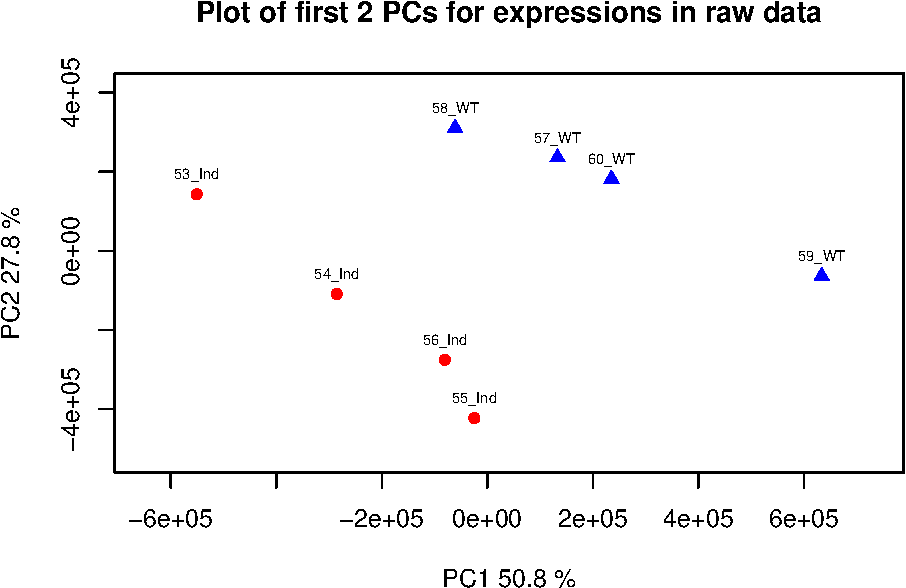
\includegraphics{APUNTS_files/figure-latex/graficosCalidad3-1.pdf}

Veiem al gràfic que PC1 explica el 50\% isegona 27\%; això és
\textgreater75\%. Els grups estan separats per una diagonal, pel que
deduïm que necessitem aquestes dues PC.

El següent chunk passa els gràfics a PDF per tenir-los per consultar
posteriorment:

\begin{Shaded}
\begin{Highlighting}[]
\CommentTok{\# SAVE TO A FILE}
\FunctionTok{pdf}\NormalTok{(}\FunctionTok{file.path}\NormalTok{(ResultsDir, }\StringTok{"QCPlots\_Raw.pdf"}\NormalTok{))  }\CommentTok{\#inicia la creació del PDF}
\CommentTok{\# ara és el codi de cada gràfic per generar en tres \textquotesingle{}pàgines\textquotesingle{} de PDF diferents.}
\FunctionTok{boxplot}\NormalTok{(rawData, }\AttributeTok{which =} \StringTok{"all"}\NormalTok{, }\AttributeTok{las =} \DecValTok{2}\NormalTok{, }\AttributeTok{main =} \StringTok{"Intensity distribution of RAW data"}\NormalTok{,}
    \AttributeTok{cex.axis =} \FloatTok{0.6}\NormalTok{, }\AttributeTok{col =}\NormalTok{ sampleColor, }\AttributeTok{names =}\NormalTok{ sampleNames)}
\FunctionTok{plot}\NormalTok{(clust.euclid.average, }\AttributeTok{labels =}\NormalTok{ sampleNames, }\AttributeTok{main =} \StringTok{"Hierarchical clustering of samples of RawData"}\NormalTok{,}
    \AttributeTok{cex =} \FloatTok{0.7}\NormalTok{, }\AttributeTok{hang =} \SpecialCharTok{{-}}\DecValTok{1}\NormalTok{)}
\FunctionTok{plotPCA}\NormalTok{(}\FunctionTok{exprs}\NormalTok{(rawData), }\AttributeTok{labels =}\NormalTok{ sampleNames, }\AttributeTok{dataDesc =} \StringTok{"raw data"}\NormalTok{, }\AttributeTok{colors =}\NormalTok{ sampleColor,}
    \AttributeTok{formapunts =} \FunctionTok{c}\NormalTok{(}\FunctionTok{rep}\NormalTok{(}\DecValTok{16}\NormalTok{, }\DecValTok{4}\NormalTok{), }\FunctionTok{rep}\NormalTok{(}\DecValTok{17}\NormalTok{, }\DecValTok{4}\NormalTok{)), }\AttributeTok{myCex =} \FloatTok{0.6}\NormalTok{)}
\FunctionTok{dev.off}\NormalTok{()  }\CommentTok{\#fi de la creació del PDF}
\end{Highlighting}
\end{Shaded}

\begin{verbatim}
pdf 
  2 
\end{verbatim}

\section{CONTROL DE QUALITAT AMB
`arrayQualityMetrics'}\label{control-de-qualitat-amb-arrayqualitymetrics}

Això ens permet fer-ho més ràpid i no gràfic per gràfic. Li donem com a
objecte el rawData i ens fa un gràfic de control de qualitat. Això sí,
tarda una mica, i no sol donar més info que el que hem fet. El profe ha
ficat una variable boleana per determinar si s'executa o no:

\begin{Shaded}
\begin{Highlighting}[]
\CommentTok{\# Avoid re{-}running it each time the script is executed.}
\NormalTok{rerun }\OtherTok{\textless{}{-}} \ConstantTok{FALSE}
\ControlFlowTok{if}\NormalTok{ (rerun) \{}
    \FunctionTok{arrayQualityMetrics}\NormalTok{(rawData, }\AttributeTok{reporttitle =} \StringTok{"QC\_RawData"}\NormalTok{, }\AttributeTok{force =} \ConstantTok{TRUE}\NormalTok{)}
\NormalTok{\}}
\end{Highlighting}
\end{Shaded}

El document generat és un html que es troba dins la carpeta que li hem
dit, en aquest cas, QC\_RawData. Dins de l'informe que es genera veiem
que hi ha una taula al principi on hi ha tres columnes que són els tres
criteris que podríen indicar que hi ha un error. El tercer és el menys
precís/eficient. El gràfic dos és per indicar si hi ha alguna mostra
atípica, que per ser-ho ha de superar la línia negra de la dreta.

\textbf{EL CONTROL DE QUALITAT ES POT DFER ABANS I DESPRÉS DE
NORMALITZAR LES DADES, PERÒ\ldots{}}

\textbf{\ldots Es recomana fer tot això abans de la normalització ja que
sinó podríem veure que la variabilitat explicada en PCA és menor. Això
és perquè es comprimeixen les dades i es redueix la variabilitat.}

\section{NORMALITZACIÓ}\label{normalitzaciuxf3}

La farem amb el mètode rma = robust multiarray average.

\begin{Shaded}
\begin{Highlighting}[]
\NormalTok{eset }\OtherTok{\textless{}{-}} \FunctionTok{rma}\NormalTok{(rawData)  }\CommentTok{\#RMA del paquet affy}
\end{Highlighting}
\end{Shaded}

\begin{verbatim}
Background correcting
Normalizing
Calculating Expression
\end{verbatim}

\begin{Shaded}
\begin{Highlighting}[]
\FunctionTok{write.exprs}\NormalTok{(eset, }\FunctionTok{file.path}\NormalTok{(ResultsDir, }\StringTok{"NormData.txt"}\NormalTok{))  }\CommentTok{\#guardar les dades en un fitxer; escriu la matriu d\textquotesingle{}expressió d\textquotesingle{}un ExpressionSet en un fitxer}
\NormalTok{eset}
\end{Highlighting}
\end{Shaded}

\begin{verbatim}
ExpressionSet (storageMode: lockedEnvironment)
assayData: 35556 features, 8 samples 
  element names: exprs 
protocolData
  rowNames: 1 2 ... 8 (8 total)
  varLabels: exprs dates
  varMetadata: labelDescription channel
phenoData
  rowNames: 1 2 ... 8 (8 total)
  varLabels: fileName grupos ShortName Colors
  varMetadata: labelDescription channel
featureData: none
experimentData: use 'experimentData(object)'
Annotation: pd.mogene.1.0.st.v1 
\end{verbatim}

Normalització quantilica: Normalitza les dades entre els diferents
arrays perquè tinguin la mateixa distribució. Les dades s'han guardat en
un arxiu dins de results per tenir-los a mà. El resultat final és un
expressionSet, que si ens fixem amb la sortida que ens dona, hi ha
assayData: \emph{ExpressionSet (storageMode: lockedEnvironment);
assayData: 35556 features, 8 samples.} S'han agrupat les sondes, ja que
si compararem amb rawdata, hi havia moltes més entrades:
\emph{GeneFeatureSet (storageMode: lockedEnvironment); assayData:
1102500 features, 8 samples.}

\section{FILTRAT}\label{filtrat}

Ara farem un filtratge dels gens per eliminar aquells amb baixa
variabilitat (si canvien poc entre els diferents grups, no ens donarà
resultats; o bé els que no tenen identificador ENTREZ). El que volem és
eliminar soroll innecessari i potenciar els resultats estadístics.

No és imprescindible tenir el paquet d'anotacions per filtrar (el
require.entrez) però si el tenim, podrem eliminar les sondes que no
estan anotades i que no solen tenir interès. Veiem al codi que fa servir
el rang interquartílic, ens quedem amb el 25\% més variable i que tenen
ID entrez.

Amb tot això guanyem un dataset menor, que té menys gens vaja, del que
hem descartat els gens que amb gran probabilitat no estaran relacionats
amb el nostre problema. Ens deixarà fer el multiple testing de manera
menys restrictiva. Avui en dia cada vegada es fa menys filtratge.

\begin{Shaded}
\begin{Highlighting}[]
\FunctionTok{annotation}\NormalTok{(rawData)}
\end{Highlighting}
\end{Shaded}

\begin{verbatim}
[1] "pd.mogene.1.0.st.v1"
\end{verbatim}

\begin{Shaded}
\begin{Highlighting}[]
\FunctionTok{library}\NormalTok{(genefilter)  }\CommentTok{\#paquet necessari per fer el filtratge}
\FunctionTok{annotation}\NormalTok{(eset) }\OtherTok{\textless{}{-}} \StringTok{"mogene10sttranscriptcluster.db"}  \CommentTok{\#assigna l\textquotesingle{}anotació \textquotesingle{}mogene10sttranscriptcluster.db\textquotesingle{} al teu objecte eset. ndica que les dades d\textquotesingle{}expressió corresponen a microarrays de ratolí (mogene) i que s\textquotesingle{}utilitzarà la base de dades \textquotesingle{}mogene10sttranscriptcluster.db\textquotesingle{} per obtenir informació sobre els gens. Aquesta info no està disponible fàcilment (has de tenir experiència amb bioconductor per deduir el paquet). Adjunto explicació AI.}
\NormalTok{eset\_filtered }\OtherTok{\textless{}{-}} \FunctionTok{nsFilter}\NormalTok{(eset, }\AttributeTok{var.func =}\NormalTok{ IQR, }\AttributeTok{var.cutoff =} \FloatTok{0.75}\NormalTok{, }\AttributeTok{var.filter =} \ConstantTok{TRUE}\NormalTok{,}
    \AttributeTok{require.entrez =} \ConstantTok{TRUE}\NormalTok{, }\AttributeTok{filterByQuantile =} \ConstantTok{TRUE}\NormalTok{)}
\CommentTok{\# NUMBER OF GENES REMOVED}
\FunctionTok{print}\NormalTok{(eset\_filtered)  }\CommentTok{\#és una llista. Si l\textquotesingle{}obrim veiem que ens diu quants ha eliminat, quants tenien poca variabilitat i quants no tenien ID ENTREZ}
\end{Highlighting}
\end{Shaded}

\begin{verbatim}
$eset
ExpressionSet (storageMode: lockedEnvironment)
assayData: 5041 features, 8 samples 
  element names: exprs 
protocolData
  rowNames: 1 2 ... 8 (8 total)
  varLabels: exprs dates
  varMetadata: labelDescription channel
phenoData
  rowNames: 1 2 ... 8 (8 total)
  varLabels: fileName grupos ShortName Colors
  varMetadata: labelDescription channel
featureData: none
experimentData: use 'experimentData(object)'
Annotation: mogene10sttranscriptcluster.db 

$filter.log
$filter.log$numDupsRemoved
[1] 1943

$filter.log$numLowVar
[1] 15123

$filter.log$numRemoved.ENTREZID
[1] 13449
\end{verbatim}

\begin{Shaded}
\begin{Highlighting}[]
\CommentTok{\# NUMBER OF GENES IN}
\FunctionTok{print}\NormalTok{(eset\_filtered}\SpecialCharTok{$}\NormalTok{eset)  }\CommentTok{\#ExpressionSet amb 5041 gens}
\end{Highlighting}
\end{Shaded}

\begin{verbatim}
ExpressionSet (storageMode: lockedEnvironment)
assayData: 5041 features, 8 samples 
  element names: exprs 
protocolData
  rowNames: 1 2 ... 8 (8 total)
  varLabels: exprs dates
  varMetadata: labelDescription channel
phenoData
  rowNames: 1 2 ... 8 (8 total)
  varLabels: fileName grupos ShortName Colors
  varMetadata: labelDescription channel
featureData: none
experimentData: use 'experimentData(object)'
Annotation: mogene10sttranscriptcluster.db 
\end{verbatim}

\subsubsection{\texorpdfstring{\textbf{Interpretació del nom de la
plataforma
(\texttt{pd.mogene.1.0.st.v1})}}{Interpretació del nom de la plataforma (pd.mogene.1.0.st.v1)}}\label{interpretaciuxf3-del-nom-de-la-plataforma-pd.mogene.1.0.st.v1}

\begin{itemize}
\item
  \textbf{\texttt{mogene}} → Es refereix al \emph{Mouse Gene} array.
\item
  \textbf{\texttt{1.0}} → La versió de l'array.
\item
  \textbf{\texttt{st}} → Significa \emph{Sense Targeted}, que indica que
  l'array utilitza sondes orientades a transcripcions completes
  (\emph{transcript clusters}).
\item
  \textbf{\texttt{v1}} → Versió de la plataforma, que no afecta
  l'anotació perquè fa referència al disseny físic.
\end{itemize}

Aquest nom indica que estàs treballant amb l'array ``Mouse Gene 1.0 ST
Array'', que fa servir \emph{transcript clusters} com a unitat
d'anotació.

\subsubsection{\texorpdfstring{\textbf{Connexió amb els paquets
d'anotació}}{Connexió amb els paquets d'anotació}}\label{connexiuxf3-amb-els-paquets-danotaciuxf3}

A Bioconductor, els paquets de bases de dades per a arrays d'Affymetrix
segueixen un patró consistent:

\begin{itemize}
\item
  Els arrays que utilitzen clústers de transcripció tenen el sufix
  \textbf{\texttt{transcriptcluster.db}}.
\item
  L'arrel del nom del paquet sempre està relacionada amb el nom de la
  plataforma (en aquest cas, \textbf{\texttt{mogene10st}}).
\end{itemize}

Això significa que:

\begin{itemize}
\item
  \textbf{\texttt{mogene10st}} és l'arrel perquè fa referència a ``Mouse
  Gene 1.0 ST Array''.
\item
  \textbf{\texttt{transcriptcluster.db}} indica que és un paquet
  d'anotació basat en clústers de transcripció.
\end{itemize}

\subsubsection{\texorpdfstring{\textbf{Absència d'informació explícita
en
Bioconductor}}{Absència d'informació explícita en Bioconductor}}\label{absuxe8ncia-dinformaciuxf3-expluxedcita-en-bioconductor}

Tot i que Bioconductor no et dóna directament aquesta associació, pots
deduir-ho:

\begin{itemize}
\item
  Les plataformes \texttt{pd.*} d'Affymetrix tenen paquets associats
  d'anotació que segueixen el mateix prefix. Per exemple:

  \begin{itemize}
  \item
    \texttt{pd.mogene.2.0.st} → \texttt{mogene20sttranscriptcluster.db}
  \item
    \texttt{pd.hugene.1.0.st.v1} →
    \texttt{hugene10sttranscriptcluster.db}
  \item
    \texttt{pd.clariom.s.mouse.ht} →
    \texttt{clariomsmousetranscriptcluster.db}
  \end{itemize}
\end{itemize}

Aquesta regularitat en els noms ajuda a deduir que:

\begin{itemize}
\tightlist
\item
  \texttt{pd.mogene.1.0.st.v1} →
  \textbf{\texttt{mogene10sttranscriptcluster.db}}
\end{itemize}

\begin{Shaded}
\begin{Highlighting}[]
\NormalTok{filteredEset }\OtherTok{\textless{}{-}}\NormalTok{ eset\_filtered}\SpecialCharTok{$}\NormalTok{eset  }\CommentTok{\#extreiem l\textquotesingle{}expressionSet}
\NormalTok{filteredData }\OtherTok{\textless{}{-}} \FunctionTok{exprs}\NormalTok{(filteredEset)  }\CommentTok{\#la matriu d\textquotesingle{}expressió}
\FunctionTok{pData}\NormalTok{(eset\_filtered}\SpecialCharTok{$}\NormalTok{eset)}\SpecialCharTok{$}\NormalTok{ShortName}
\end{Highlighting}
\end{Shaded}

\begin{verbatim}
[1] "53_Ind" "54_Ind" "55_Ind" "56_Ind" "57_WT"  "58_WT"  "59_WT"  "60_WT" 
\end{verbatim}

\begin{Shaded}
\begin{Highlighting}[]
\FunctionTok{colnames}\NormalTok{(filteredData) }\OtherTok{\textless{}{-}} \FunctionTok{pData}\NormalTok{(eset\_filtered}\SpecialCharTok{$}\NormalTok{eset)}\SpecialCharTok{$}\NormalTok{ShortName  }\CommentTok{\#canviem el nom de les columnes, així tindrem les etiquetes posteriorment.}
\end{Highlighting}
\end{Shaded}

\section{SELECCIÓ DE GENS}\label{selecciuxf3-de-gens}

En aquest cas tenim únicament dos grups (inudït/no induït) i un factor a
analitzar. Farem servir el programa LIMMA; aquest ens proporciona una
gran quantitat d'informació com ara un estimador de la variabilitat de
cada gen. Aqust càlcul el fa mirant la variabilitat de cada gen vs la
variabilitat global del dataset.

Primer construïrem una matriu de disseny. Podem utilitzar
\emph{modelmatrix} indicant quin factor volem que es faci servir. La
matriu de disseny és una representació matemàtica de l'estructura
experimental que s'utilitza per modelar les dades i identificar els gens
que canvien la seva expressió entre les condicions experimentals.

\begin{Shaded}
\begin{Highlighting}[]
\FunctionTok{library}\NormalTok{(limma)}
\FunctionTok{pData}\NormalTok{(filteredEset)}\SpecialCharTok{$}\NormalTok{grupos}
\end{Highlighting}
\end{Shaded}

\begin{verbatim}
[1] "Induced" "Induced" "Induced" "Induced" "WT"      "WT"      "WT"     
[8] "WT"     
\end{verbatim}

\begin{Shaded}
\begin{Highlighting}[]
\NormalTok{treat }\OtherTok{\textless{}{-}} \FunctionTok{pData}\NormalTok{(filteredEset)}\SpecialCharTok{$}\NormalTok{grupos  }\CommentTok{\#extreiem la columna de gups de les metadades i ho guardem dins la varaible treat}
\NormalTok{lev }\OtherTok{\textless{}{-}} \FunctionTok{factor}\NormalTok{(treat, }\AttributeTok{levels =} \FunctionTok{unique}\NormalTok{(treat))  }\CommentTok{\#fem que sigui factor. La part de levels assegura que els nivells del factors sigui únics i presents de la var treat.}
\NormalTok{design }\OtherTok{\textless{}{-}} \FunctionTok{model.matrix}\NormalTok{(}\SpecialCharTok{\textasciitilde{}}\DecValTok{0} \SpecialCharTok{+}\NormalTok{ lev)  }\CommentTok{\#0 indica que no es vol incloure un terme d\textquotesingle{}intercepció al model, i lev indica que es vol incloure una columna per a cada nivell del factor lev.}
\FunctionTok{colnames}\NormalTok{(design) }\OtherTok{\textless{}{-}} \FunctionTok{levels}\NormalTok{(lev)}
\FunctionTok{rownames}\NormalTok{(design) }\OtherTok{\textless{}{-}}\NormalTok{ sampleNames}
\CommentTok{\# La matriu de disseny resultant tindrà una fila per a cada mostra i una}
\CommentTok{\# columna per a cada grup experimental. Els valors de la matriu seran 1 si la}
\CommentTok{\# mostra pertany al grup corresponent i 0 en cas contrari.}
\FunctionTok{print}\NormalTok{(design)}
\end{Highlighting}
\end{Shaded}

\begin{verbatim}
       Induced WT
53_Ind       1  0
54_Ind       1  0
55_Ind       1  0
56_Ind       1  0
57_WT        0  1
58_WT        0  1
59_WT        0  1
60_WT        0  1
attr(,"assign")
[1] 1 1
attr(,"contrasts")
attr(,"contrasts")$lev
[1] "contr.treatment"
\end{verbatim}

Ara fem la matriu de contrast = consisteix en dir quines comparacions
volem fer en forma de resta: induïts vs no afectat.

\begin{Shaded}
\begin{Highlighting}[]
\CommentTok{\#COMPARISON}
\NormalTok{cont.matrix1 }\OtherTok{\textless{}{-}} \FunctionTok{makeContrasts}\NormalTok{(  }\CommentTok{\#la funció makeConstrasts és la que fa la matriu.}
        \AttributeTok{Induced.vs.WT =}\NormalTok{ Induced}\SpecialCharTok{{-}}\NormalTok{WT,}\CommentTok{\#induced vs wild type}
        \AttributeTok{levels =}\NormalTok{ design) }\CommentTok{\#els nivells han de ser els mateixos que els de la matriu anterior}
\NormalTok{comparisonName }\OtherTok{\textless{}{-}} \StringTok{"Efecto de la Inducción"} \CommentTok{\#Assigna el nom "Efecto de la Inducción" a una variable anomenada comparisonName}
\FunctionTok{print}\NormalTok{(cont.matrix1)}
\end{Highlighting}
\end{Shaded}

\begin{verbatim}
         Contrasts
Levels    Induced.vs.WT
  Induced             1
  WT                 -1
\end{verbatim}

Ara estimarem el model. Amb el paquet limma ara ajustem un model lineal
a les dades d'expressió filtrades i calculem estadísiques per a la
comparació de grups. Així podrem identificar els gens que canvien
significativament la seva expressió entre les condicions experimentals.

\begin{Shaded}
\begin{Highlighting}[]
\CommentTok{\# MODEL FIT}
\NormalTok{fit1 }\OtherTok{\textless{}{-}} \FunctionTok{lmFit}\NormalTok{(filteredData, design)  }\CommentTok{\#ajustem el model fent servir les dades d\textquotesingle{}expressió filteredData i la matriu de disseny design.}
\NormalTok{fit.main1 }\OtherTok{\textless{}{-}} \FunctionTok{contrasts.fit}\NormalTok{(fit1, cont.matrix1)  }\CommentTok{\#aplica la matriu de contrasts a fit1 per fer les estadístiques de comparació.}
\NormalTok{fit.main1 }\OtherTok{\textless{}{-}} \FunctionTok{eBayes}\NormalTok{(fit.main1)  }\CommentTok{\#Calcula estadístiques moderades utilitzant un mètode empíric Bayes. eBayes=bayes empíric}
\end{Highlighting}
\end{Shaded}

Hi ha alternatives vàlides al mètode empíric Bayes utilitzat en el
paquet \texttt{limma} per a l'anàlisi d'expressió diferencial. Algunes
d'aquestes alternatives inclouen:

\begin{itemize}
\item
  \textbf{t-test:} El t-test és una prova estadística clàssica que es
  pot utilitzar per comparar les mitjanes de dos grups. Es pot utilitzar
  per a l'anàlisi d'expressió diferencial quan es comparen dos grups
  experimentals.
\item
  \textbf{ANOVA:} L'ANOVA (anàlisi de la variància) és una prova
  estadística que es pot utilitzar per comparar les mitjanes de tres o
  més grups. Es pot utilitzar per a l'anàlisi d'expressió diferencial
  quan es comparen múltiples grups experimentals.
\item
  \textbf{SAM (Significance Analysis of Microarrays):} SAM és un mètode
  estadístic no paramètric que es va desenvolupar específicament per a
  l'anàlisi d'expressió diferencial de microarrays.
\item
  \textbf{Rank product:} El mètode de rank product és un altre mètode no
  paramètric que es pot utilitzar per a l'anàlisi d'expressió
  diferencial.
\end{itemize}

Per exemple, el t-test i l'ANOVA són mètodes clàssics que són fàcils
d'implementar i interpretar, però poden ser menys potents que el mètode
empíric Bayes quan el nombre de mostres és petit. SAM i el mètode de
rank product són mètodes no paramètrics que són més robustos a la
presència de valors atípics, però poden ser més difícils d'implementar.

Els resultats de l'anàlisi que hem fet estan guardats dins l'objecte
\texttt{lmfit} i es poden extreure amb la instrucció \texttt{topTable}.
Aquesta instrucció, \texttt{topTable}, pot aplicar un filtre automàtic
basat en dos criteris diferents: ``log fold change'' i ``p-value''. En
aquest cas agafarem únicament els gens amb un log-fold-change més gran
de 3 i p-valor ajustat inferior a 0.05.

\begin{Shaded}
\begin{Highlighting}[]
\NormalTok{topTab }\OtherTok{\textless{}{-}} \FunctionTok{topTable}\NormalTok{(fit.main1, }\AttributeTok{number =} \FunctionTok{nrow}\NormalTok{(fit.main1), }\AttributeTok{coef =} \StringTok{"Induced.vs.WT"}\NormalTok{, }\AttributeTok{adjust =} \StringTok{"fdr"}\NormalTok{,}
    \AttributeTok{lfc =} \DecValTok{3}\NormalTok{, }\AttributeTok{p.value =} \FloatTok{0.05}\NormalTok{)}
\CommentTok{\# de fitmain1 treiem les estadístiques. number{-}{-}\textgreater{}indica que es volen mostrar}
\CommentTok{\# tots els gens. coef = \textquotesingle{}Induced.vs.WT\textquotesingle{}: Especifica el contrast per al qual es}
\CommentTok{\# volen extreure els DEGs. adjust = \textquotesingle{}fdr\textquotesingle{}: Indica que es vol ajustar el p{-}valor}
\CommentTok{\# per controlar la taxa de falsos descobriments (FDR). lfc = 3: Especifica un}
\CommentTok{\# log fold change (lfc) mínim de 3 per considerar un gen com a diferencialment}
\CommentTok{\# expressat. Això significa que només es mostraran els gens que tenen un canvi}
\CommentTok{\# d\textquotesingle{}expressió de almenys 3 vegades (en escala logarítmica) entre els grups.}
\CommentTok{\# p.value = 0.05: Especifica un p{-}valor màxim de 0.05 per considerar un gen com}
\CommentTok{\# a diferencialment expressat.}
\FunctionTok{dim}\NormalTok{(topTab)}
\end{Highlighting}
\end{Shaded}

\begin{verbatim}
[1] 219   6
\end{verbatim}

\begin{Shaded}
\begin{Highlighting}[]
\FunctionTok{head}\NormalTok{(topTab)}
\end{Highlighting}
\end{Shaded}

\begin{verbatim}
             logFC  AveExpr         t      P.Value    adj.P.Val        B
10470175  5.707416 7.364107  37.97989 1.509750e-12 5.098562e-09 18.94789
10351443  5.779825 9.600246  36.92502 2.022838e-12 5.098562e-09 18.71043
10403796  5.654198 8.316620  34.73894 3.811235e-12 6.331269e-09 18.18482
10522388  5.531318 8.431707  33.36608 5.790093e-12 6.331269e-09 17.82961
10469358 -5.371210 7.747743 -33.10581 6.279775e-12 6.331269e-09 17.75992
10531869  5.751976 8.785049  31.78481 9.576493e-12 7.061047e-09 17.39403
\end{verbatim}

L'estadístic B és un resultat bayesià de la probabilitat que estigui
diferencialment expressat vs que no.

\section{ANOTACIÓ DE RESULTATS}\label{anotaciuxf3-de-resultats}

Ara el que farem és obtenir els identificadors dels gens que ens
interessen. Això ho farem obtenint els identiicadors de ENTREZ i GENE
SYMBOL corresponents als probesets que hi ha a la taula de resultats
(identificats amb els id de la companyia que ha produït els
microarrays).

\begin{Shaded}
\begin{Highlighting}[]
\FunctionTok{library}\NormalTok{(mogene10sttranscriptcluster.db)  }\CommentTok{\#carreguem el paquet d\textquotesingle{}anotació. }
\FunctionTok{keytypes}\NormalTok{(mogene10sttranscriptcluster.db)  }\CommentTok{\#ens ensenya els tipus de claus disponibles. }
\end{Highlighting}
\end{Shaded}

\begin{verbatim}
 [1] "ACCNUM"       "ALIAS"        "ENSEMBL"      "ENSEMBLPROT"  "ENSEMBLTRANS"
 [6] "ENTREZID"     "ENZYME"       "EVIDENCE"     "EVIDENCEALL"  "GENENAME"    
[11] "GENETYPE"     "GO"           "GOALL"        "IPI"          "MGI"         
[16] "ONTOLOGY"     "ONTOLOGYALL"  "PATH"         "PFAM"         "PMID"        
[21] "PROBEID"      "PROSITE"      "REFSEQ"       "SYMBOL"       "UNIPROT"     
\end{verbatim}

\begin{Shaded}
\begin{Highlighting}[]
\NormalTok{anotaciones }\OtherTok{\textless{}{-}}\NormalTok{ AnnotationDbi}\SpecialCharTok{::}\FunctionTok{select}\NormalTok{(mogene10sttranscriptcluster.db, }\AttributeTok{keys =} \FunctionTok{rownames}\NormalTok{(filteredData),}
    \AttributeTok{columns =} \FunctionTok{c}\NormalTok{(}\StringTok{"ENTREZID"}\NormalTok{, }\StringTok{"SYMBOL"}\NormalTok{))  }\CommentTok{\#obtenim les anotacions amb select; les claus són els noms de la fila de la matriu filteredDAta; li diem les columnes que volem extreure. Ho guardem tot a anotaciones. }
\NormalTok{anotaciones}
\end{Highlighting}
\end{Shaded}

\begin{verbatim}
    PROBEID  ENTREZID        SYMBOL
1  10379727 100034251        Wfdc17
2  10585180 100036537       Gm11149
3  10554156 100038347       Fam174b
4  10408047 100038371        Zfp389
5  10500360 100038464       Gm15441
6  10578950 100038489         Apela
7  10405892 100038538        Ramacl
8  10436692 100038614       Gm10791
9  10352794 100038712       Gm10516
10 10369102 100038725        Cep85l
11 10453555 100038746        Gm1976
12 10362102 100038752       Gm10825
13 10451287 100038882         Isg15
14 10406823 100039691       Lncenc1
15 10362534 100040846 5930403N24Rik
16 10368700 100041085    Mfsd4b3-ps
17 10402783 100041194        Ahnak2
18 10490843 100041480        Myef2l
19 10505163 100041581      Zkscan16
20 10412488 100041678        Gm3500
21 10523750 100042165        Thoc2l
22 10414747 100043218     Trav12n-1
23 10558400 100043254           Nps
24 10487506 100043424       Morrbid
25 10486201 100043609       Gm14207
 [ reached 'max' / getOption("max.print") -- omitted 5016 rows ]
\end{verbatim}

Habitualment es fa servir entrez, ensembl i symbol, que aquest últim no
és tan estàndard però és més intuïtiu.

Ara afegirem aquesta informació a topTable. Per fer-ho, fa servir
concatenació fent servir ``pipes'' del paquet dyplr:

\begin{Shaded}
\begin{Highlighting}[]
\FunctionTok{library}\NormalTok{(dplyr)}
\NormalTok{topTabAnotada }\OtherTok{\textless{}{-}}\NormalTok{ topTab }\SpecialCharTok{\%\textgreater{}\%}  \CommentTok{\#està creant una nova taula; \%\textgreater{}\% anotador pipe que ens deixa fer múltiples operacions a la vegada}
  \FunctionTok{mutate}\NormalTok{(}\AttributeTok{PROBEID=}\FunctionTok{rownames}\NormalTok{(topTab)) }\SpecialCharTok{\%\textgreater{}\%} \CommentTok{\#afegeix una nova columna}
  \FunctionTok{left\_join}\NormalTok{(anotaciones) }\SpecialCharTok{\%\textgreater{}\%} \CommentTok{\#combina les taules utiltizant unió oper l\textquotesingle{}esquerra}
  \FunctionTok{arrange}\NormalTok{(P.Value) }\SpecialCharTok{\%\textgreater{}\%} \CommentTok{\#reordena el p valor en ordre descendent. }
  \FunctionTok{select}\NormalTok{(}\DecValTok{7}\NormalTok{,}\DecValTok{8}\NormalTok{,}\DecValTok{9}\NormalTok{, }\DecValTok{1}\SpecialCharTok{:}\DecValTok{6}\NormalTok{) }\CommentTok{\#reordena les columnes:  Primer es mostren les columnes 7, 8 i 9 (que corresponen a "PROBEID", "ENTREZID" i "SYMBOL"), seguides de les columnes 1 a 6 (que contenen la resta d\textquotesingle{}informació sobre els gens diferencialment expressats).}

\FunctionTok{head}\NormalTok{(topTabAnotada)}
\end{Highlighting}
\end{Shaded}

\begin{verbatim}
   PROBEID ENTREZID  SYMBOL     logFC  AveExpr         t      P.Value
1 10470175   227627   Obp2a  5.707416 7.364107  37.97989 1.509750e-12
2 10351443   110648   Lmx1a  5.779825 9.600246  36.92502 2.022838e-12
3 10403796   218038    Amph  5.654198 8.316620  34.73894 3.811235e-12
4 10522388   231290 Slc10a4  5.531318 8.431707  33.36608 5.790093e-12
5 10469358    17533    Mrc1 -5.371210 7.747743 -33.10581 6.279775e-12
6 10531869    26414  Mapk10  5.751976 8.785049  31.78481 9.576493e-12
     adj.P.Val        B
1 5.098562e-09 18.94789
2 5.098562e-09 18.71043
3 6.331269e-09 18.18482
4 6.331269e-09 17.82961
5 6.331269e-09 17.75992
6 7.061047e-09 17.39403
\end{verbatim}

Amb aquests resultats, generem un nou document per tenir-lo.

\begin{Shaded}
\begin{Highlighting}[]
\FunctionTok{write.csv2}\NormalTok{(topTabAnotada, }\AttributeTok{file =} \FunctionTok{file.path}\NormalTok{(ResultsDir, }\StringTok{"Genes seleccionados.csv"}\NormalTok{))}
\FunctionTok{print}\NormalTok{(}\FunctionTok{xtable}\NormalTok{(topTab, }\AttributeTok{align =} \StringTok{"lllllll"}\NormalTok{), }\AttributeTok{type =} \StringTok{"html"}\NormalTok{, }\AttributeTok{html.table.attributes =} \StringTok{""}\NormalTok{,}
    \AttributeTok{file =} \FunctionTok{file.path}\NormalTok{(ResultsDir, }\StringTok{"Genes seleccionados.html"}\NormalTok{))}
\end{Highlighting}
\end{Shaded}

\section{VISUALITZACIÓ DELS
RESULTATS}\label{visualitzaciuxf3-dels-resultats}

Podem fer un volcano plot o bé un heat map.

\subsection{VOLCANO PLOT}\label{volcano-plot}

El volcano plot és un tipus de gràfic que mostra el log fold change
(lfc) a l'eix x i el -log10 del p-valor a l'eix y. Això permet
identificar fàcilment els gens que tenen un canvi d'expressió
significatiu i un p-valor baix.

\begin{Shaded}
\begin{Highlighting}[]
\NormalTok{genenames }\OtherTok{\textless{}{-}}\NormalTok{ AnnotationDbi}\SpecialCharTok{::}\FunctionTok{select}\NormalTok{(mogene10sttranscriptcluster.db, }\FunctionTok{rownames}\NormalTok{(fit.main1),}
    \FunctionTok{c}\NormalTok{(}\StringTok{"SYMBOL"}\NormalTok{))}\SpecialCharTok{$}\NormalTok{SYMBOL  }\CommentTok{\#agafem els noms del paquet que hem fet servir fins ara. Rownames els agafem de fit.main1 que són els identificadors de les sondes. Volem extreure el símbol. Ho guardem a genenames.}
\FunctionTok{volcanoplot}\NormalTok{(fit.main1, }\AttributeTok{highlight =} \DecValTok{10}\NormalTok{, }\AttributeTok{names =}\NormalTok{ genenames, }\AttributeTok{main =} \FunctionTok{paste}\NormalTok{(}\StringTok{"Differentially expressed genes"}\NormalTok{,}
    \FunctionTok{colnames}\NormalTok{(cont.matrix1), }\AttributeTok{sep =} \StringTok{"}\SpecialCharTok{\textbackslash{}n}\StringTok{"}\NormalTok{))}
\FunctionTok{abline}\NormalTok{(}\AttributeTok{v =} \FunctionTok{c}\NormalTok{(}\SpecialCharTok{{-}}\DecValTok{3}\NormalTok{, }\DecValTok{3}\NormalTok{))  }\CommentTok{\#línia per veure el logfold}
\end{Highlighting}
\end{Shaded}

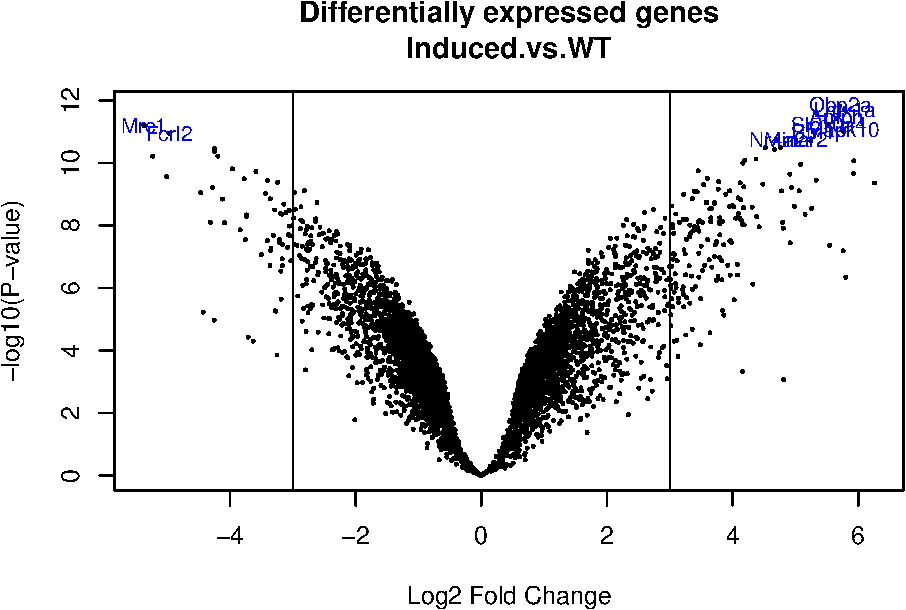
\includegraphics{APUNTS_files/figure-latex/volcanoPlot-1.pdf}

\begin{Shaded}
\begin{Highlighting}[]
\CommentTok{\# fitmain1: conté les estadístiques moderades per a la comparació entre grups;}
\CommentTok{\# donem noms només als 10 més diferents.}

\FunctionTok{pdf}\NormalTok{(}\FunctionTok{file.path}\NormalTok{(ResultsDir, }\StringTok{"Volcanos.pdf"}\NormalTok{))  }\CommentTok{\#en fem un PDF.}
\FunctionTok{volcanoplot}\NormalTok{(fit.main1, }\AttributeTok{highlight =} \DecValTok{10}\NormalTok{, }\AttributeTok{names =}\NormalTok{ genenames, }\AttributeTok{main =} \FunctionTok{paste}\NormalTok{(}\StringTok{"Differentially expressed genes"}\NormalTok{,}
    \FunctionTok{colnames}\NormalTok{(cont.matrix1), }\AttributeTok{sep =} \StringTok{"}\SpecialCharTok{\textbackslash{}n}\StringTok{"}\NormalTok{))}
\FunctionTok{abline}\NormalTok{(}\AttributeTok{v =} \FunctionTok{c}\NormalTok{(}\SpecialCharTok{{-}}\DecValTok{3}\NormalTok{, }\DecValTok{3}\NormalTok{))}
\FunctionTok{dev.off}\NormalTok{()}
\end{Highlighting}
\end{Shaded}

\begin{verbatim}
pdf 
  2 
\end{verbatim}

\subsection{HEATMAPS}\label{heatmaps}

Ara farem servir LA MATIRU D'EXPRESSIÓ.

\begin{Shaded}
\begin{Highlighting}[]
\NormalTok{selectedRows }\OtherTok{\textless{}{-}} \FunctionTok{rownames}\NormalTok{(filteredData) }\SpecialCharTok{\%in\%} \FunctionTok{rownames}\NormalTok{(topTab) }\CommentTok{\#un vector lògic selectedRows que indica quines files de la matriu filteredData corresponen als gens presents a la taula topTab (els DEGs).}
\NormalTok{selectedData }\OtherTok{\textless{}{-}}\NormalTok{ filteredData[selectedRows,]}\CommentTok{\#una nova matriu selectedData que conté només les files de filteredData que corresponen als DEGs.}

\CommentTok{\#HEATMAP PLOT}
\NormalTok{my\_palette }\OtherTok{\textless{}{-}} \FunctionTok{colorRampPalette}\NormalTok{(}\FunctionTok{c}\NormalTok{(}\StringTok{"blue"}\NormalTok{, }\StringTok{"red"}\NormalTok{))(}\AttributeTok{n =} \DecValTok{299}\NormalTok{) }\CommentTok{\#paleta de colors que va del blau al vermell amb 299 colors intermedis. }
\FunctionTok{library}\NormalTok{(gplots)}
\FunctionTok{heatmap.2}\NormalTok{(selectedData,}
          \AttributeTok{Rowv=}\ConstantTok{TRUE}\NormalTok{, }\CommentTok{\#agrupa gens}
          \AttributeTok{Colv=}\ConstantTok{TRUE}\NormalTok{, }\CommentTok{\#agrupa columnes}
          \AttributeTok{main=}\StringTok{"HeatMap Induced.vs.WT FC\textgreater{}=3"}\NormalTok{,}
          \AttributeTok{scale=}\StringTok{"row"}\NormalTok{, }\CommentTok{\#escala valors d\textquotesingle{}expressió per fila}
          \AttributeTok{col=}\NormalTok{my\_palette,}
          \AttributeTok{sepcolor=}\StringTok{"white"}\NormalTok{,}
          \AttributeTok{sepwidth=}\FunctionTok{c}\NormalTok{(}\FloatTok{0.05}\NormalTok{,}\FloatTok{0.05}\NormalTok{),}
          \AttributeTok{cexRow=}\FloatTok{0.5}\NormalTok{,}
          \AttributeTok{cexCol=}\FloatTok{0.9}\NormalTok{,}
          \AttributeTok{key=}\ConstantTok{TRUE}\NormalTok{, }\CommentTok{\#mostra llegenda}
          \AttributeTok{keysize=}\FloatTok{1.5}\NormalTok{,}
          \AttributeTok{density.info=}\StringTok{"histogram"}\NormalTok{,}
          \AttributeTok{ColSideColors=}\FunctionTok{c}\NormalTok{(}\FunctionTok{rep}\NormalTok{(}\StringTok{"red"}\NormalTok{,}\DecValTok{4}\NormalTok{),}\FunctionTok{rep}\NormalTok{(}\StringTok{"blue"}\NormalTok{,}\DecValTok{4}\NormalTok{)), }\CommentTok{\#colors per marcar els grups experimentals}
          \AttributeTok{tracecol=}\ConstantTok{NULL}\NormalTok{,}
          \AttributeTok{srtCol=}\DecValTok{30}\NormalTok{) }\CommentTok{\#rota etiquetes}
\end{Highlighting}
\end{Shaded}

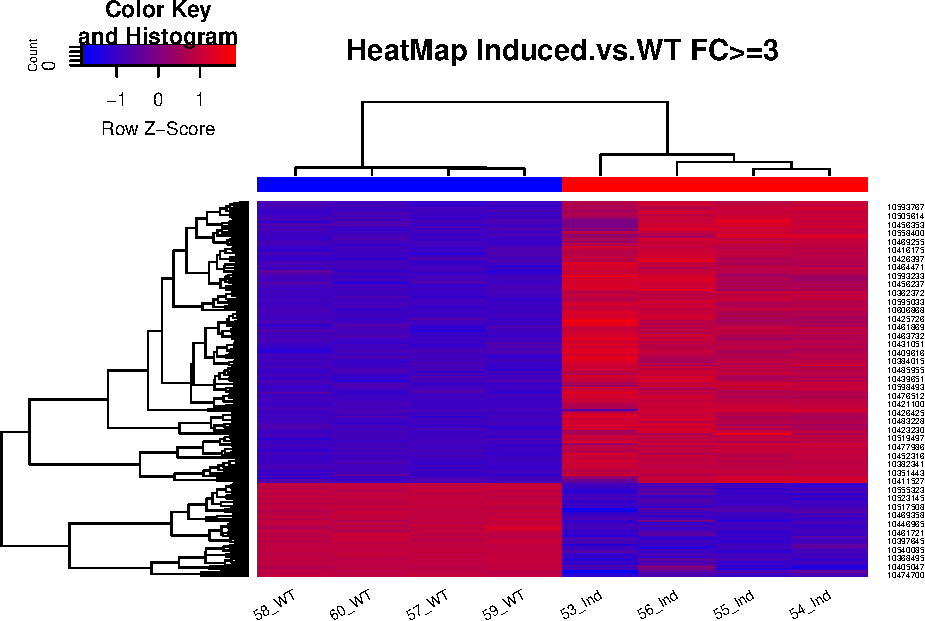
\includegraphics{APUNTS_files/figure-latex/heatmap-1.pdf}

\begin{Shaded}
\begin{Highlighting}[]
\CommentTok{\#creem el PDF}
\FunctionTok{pdf}\NormalTok{(}\FunctionTok{file.path}\NormalTok{(ResultsDir,}\StringTok{"Heatmap.pdf"}\NormalTok{))}
\FunctionTok{heatmap.2}\NormalTok{(selectedData,}
          \AttributeTok{Rowv=}\ConstantTok{TRUE}\NormalTok{,}
          \AttributeTok{Colv=}\ConstantTok{TRUE}\NormalTok{,}
          \AttributeTok{main=}\StringTok{"HeatMap Induced.vs.WT FC\textgreater{}=3"}\NormalTok{,}
          \AttributeTok{scale=}\StringTok{"row"}\NormalTok{,}
          \AttributeTok{col=}\NormalTok{my\_palette,}
          \AttributeTok{sepcolor=}\StringTok{"white"}\NormalTok{,}
          \AttributeTok{sepwidth=}\FunctionTok{c}\NormalTok{(}\FloatTok{0.05}\NormalTok{,}\FloatTok{0.05}\NormalTok{),}
          \AttributeTok{cexRow=}\FloatTok{0.5}\NormalTok{,}
          \AttributeTok{cexCol=}\FloatTok{0.9}\NormalTok{,}
          \AttributeTok{key=}\ConstantTok{TRUE}\NormalTok{,}
          \AttributeTok{keysize=}\FloatTok{1.5}\NormalTok{,}
          \AttributeTok{density.info=}\StringTok{"histogram"}\NormalTok{,}
          \AttributeTok{ColSideColors=}\FunctionTok{c}\NormalTok{(}\FunctionTok{rep}\NormalTok{(}\StringTok{"red"}\NormalTok{,}\DecValTok{4}\NormalTok{),}\FunctionTok{rep}\NormalTok{(}\StringTok{"blue"}\NormalTok{,}\DecValTok{4}\NormalTok{)),}
          \AttributeTok{tracecol=}\ConstantTok{NULL}\NormalTok{,}
          \AttributeTok{srtCol=}\DecValTok{30}\NormalTok{)}
\FunctionTok{dev.off}\NormalTok{()}
\end{Highlighting}
\end{Shaded}

\begin{verbatim}
pdf 
  2 
\end{verbatim}

Hi ha dos grups de gens: uns, els vermells, que estan menys expressats
en el wild type i més a l'induït; i uns al revés. Hem seleccionat
expressament els més expressats, per tant, el gràfic és purament
confirmatiu.

\section{ANÀLISI DE SIGNIFICACIÓ
BIOLÒGICA}\label{anuxe0lisi-de-significaciuxf3-bioluxf2gica}

Fan un anàlisi de sobre-representació, que busca si entre les anotacions
hi ha alguna categoria (amb gene onthology o així) que apareixi amb més
freqüència que la real esperada.

Per fer això necessitem:

\begin{itemize}
\item
  Una llista seleccionada.
\item
  L'univers de gens, és a dir, tots els gens que s'han inclós a
  l'anàlisi (depenent de l'usuari es posen tots els del xip o tots els
  del genoma).
\end{itemize}

La majoria de programes necessites que els identificadors dels gens
siguin format \texttt{ENTREZ}, pel que prepararem ambdues llistes a la
vegada (tot i que ja teníem la dels gens seleccionats).

\begin{Shaded}
\begin{Highlighting}[]
\FunctionTok{library}\NormalTok{(mogene10sttranscriptcluster.db)  }\CommentTok{\#carreguem el paquet d\textquotesingle{}anotació }
\NormalTok{probesUniverse }\OtherTok{\textless{}{-}} \FunctionTok{rownames}\NormalTok{(filteredData)  }\CommentTok{\#vector que conté els noms de la fila de la matriu fileData. Són els noms dels identificadors de les sondes de microarray i són l\textquotesingle{}univers de gens.}
\NormalTok{entrezUniverse }\OtherTok{\textless{}{-}}\NormalTok{ AnnotationDbi}\SpecialCharTok{::}\FunctionTok{select}\NormalTok{(mogene10sttranscriptcluster.db, probesUniverse,}
    \StringTok{"ENTREZID"}\NormalTok{)}\SpecialCharTok{$}\NormalTok{ENTREZID}
\CommentTok{\# agafem els ID d\textquotesingle{}entrez.}
\NormalTok{topProbes }\OtherTok{\textless{}{-}} \FunctionTok{rownames}\NormalTok{(selectedData)  }\CommentTok{\#les claus que s\textquotesingle{}utilitzaran per identificar els gens.}
\NormalTok{entrezTop }\OtherTok{\textless{}{-}}\NormalTok{ AnnotationDbi}\SpecialCharTok{::}\FunctionTok{select}\NormalTok{(mogene10sttranscriptcluster.db, topProbes, }\StringTok{"ENTREZID"}\NormalTok{)}\SpecialCharTok{$}\NormalTok{ENTREZID}

\NormalTok{topGenes }\OtherTok{\textless{}{-}}\NormalTok{ entrezTop[}\SpecialCharTok{!}\FunctionTok{duplicated}\NormalTok{(entrezTop)]  }\CommentTok{\#Elimina els IDs d\textquotesingle{}Entrez duplicats del vector entrezTop i emmagatzema el resultat en un vector anomenat topGenes}
\NormalTok{entrezUniverse }\OtherTok{\textless{}{-}}\NormalTok{ entrezUniverse[}\SpecialCharTok{!}\FunctionTok{duplicated}\NormalTok{(entrezUniverse)]  }\CommentTok{\#Elimina els IDs d\textquotesingle{}Entrez duplicats del vector entrezUniverse}
\end{Highlighting}
\end{Shaded}

Hi ha múltiples paquets per fer l'anàlisi d'enriquiment genètic. Cada
paquet fa coses diferents però les idees subjacents són les mateixes.

En aquest cas veurem \texttt{GEOstats}; és un dels primers paquets
disponibles de Bioconductor per fer l'anàlisi d'enriquiment. Per fer-lo
servir s'ha de crear un objecte anomenat ``hiperparàmentre'' que pot ser
de classe tipus:

\begin{itemize}
\tightlist
\item
  \texttt{GOHyperGParams} farà l'anàlisi basat en Gene Ontology.
\item
  \texttt{KEGGHyperGParams} anàlisi basat en la base de dades REACTOMA
\item
  \texttt{PFAMHyperGParams} basat en la base de dades de PFAM.
\end{itemize}

\begin{Shaded}
\begin{Highlighting}[]
\FunctionTok{library}\NormalTok{(GOstats)  }\CommentTok{\#carreguem el paquet}
\CommentTok{\# L\textquotesingle{}objecte GOHyperGParams té un argument ontology que pot ser \textquotesingle{}BP\textquotesingle{} {-}}
\CommentTok{\# biological process, \textquotesingle{}MF\textquotesingle{}{-}molecular function o \textquotesingle{}CC\textquotesingle{}{-}cellular component.}
\NormalTok{GOparams }\OtherTok{=} \FunctionTok{new}\NormalTok{(}\StringTok{"GOHyperGParams"}\NormalTok{, }\AttributeTok{geneIds =}\NormalTok{ topGenes, }\AttributeTok{universeGeneIds =}\NormalTok{ entrezUniverse,}
    \AttributeTok{annotation =} \StringTok{"mogene10sttranscriptcluster.db"}\NormalTok{, }\AttributeTok{ontology =} \StringTok{"BP"}\NormalTok{, }\AttributeTok{pvalueCutoff =} \FloatTok{0.01}\NormalTok{)}
\CommentTok{\# creem un objecte amb els IDs de topGenes, els de l\textquotesingle{}univers, fem l\textquotesingle{}anàlisi amb}
\CommentTok{\# biological process i el llindar estadístic el posem a 0.01.  S\textquotesingle{}hauria de fer}
\CommentTok{\# per a cada ontologia.}
\end{Highlighting}
\end{Shaded}

\begin{Shaded}
\begin{Highlighting}[]
\NormalTok{GOhyper }\OtherTok{=} \FunctionTok{hyperGTest}\NormalTok{(GOparams)}
\end{Highlighting}
\end{Shaded}

Executem el test i guardem el resultat a GOhyper. Aquest objecte conté
ID del terme GO, Nom del terme GO, p-valor (de la prova hipergeomètrica;
indica significació de l'enriquiment), nombre de gens, nombre esperat de
gens (nombre de gens que s'esperaria que estiguessin associats al terme
GO per atzar) i odds ratio (indica la magnitud de l'enriquiment). El
test hipergeomètric és un test de fisher.

\begin{Shaded}
\begin{Highlighting}[]
\FunctionTok{head}\NormalTok{(}\FunctionTok{summary}\NormalTok{(GOhyper))}
\end{Highlighting}
\end{Shaded}

\begin{verbatim}
      GOBPID       Pvalue OddsRatio ExpCount Count Size
1 GO:0007154 7.355197e-12  2.637205 82.00494   130 1890
2 GO:0023052 8.449083e-12  2.627972 81.18055   129 1871
3 GO:0007610 6.866247e-09  3.437609 13.36377    37  308
4 GO:0007186 1.624698e-08  3.500490 11.97532    34  276
5 GO:0007218 5.528504e-08 14.415423  1.12811    10   26
6 GO:0007165 7.638344e-08  2.128321 72.19905   109 1664
                                          Term
1                           cell communication
2                                    signaling
3                                     behavior
4 G protein-coupled receptor signaling pathway
5               neuropeptide signaling pathway
6                          signal transduction
\end{verbatim}

\begin{Shaded}
\begin{Highlighting}[]
\FunctionTok{dim}\NormalTok{(}\FunctionTok{summary}\NormalTok{(GOhyper))}
\end{Highlighting}
\end{Shaded}

\begin{verbatim}
[1] 242   7
\end{verbatim}

La primera columna ens ensenya quina categoria de la GO està més
enriquida, quantes vegades més abundant és respecte el que esperaríem
(OR=1, igual d'abundant).

Gravem els resultats.

\begin{Shaded}
\begin{Highlighting}[]
\CommentTok{\# Creamos un informe html con los resultados}
\NormalTok{GOfilename }\OtherTok{=} \FunctionTok{file.path}\NormalTok{(ResultsDir, }\StringTok{"GOResults.html"}\NormalTok{)}
\FunctionTok{htmlReport}\NormalTok{(GOhyper, }\AttributeTok{file =}\NormalTok{ GOfilename, }\AttributeTok{summary.args =} \FunctionTok{list}\NormalTok{(}\AttributeTok{htmlLinks =} \ConstantTok{TRUE}\NormalTok{))}
\end{Highlighting}
\end{Shaded}

Una vegada finalitzat l'anàlisi recomana el profe recòrrer tot el
document des de zero per a assegurar-nos que el codi és reproduïble.

Per tant, al final què tenim? A dins de la carpeta de resultats tenim:

\begin{itemize}
\item
  Els gens que estan diferencialment expressats (topTable)
\item
  Resultats de significació biològica
\item
  Gràfics de control de qualitat
\item
  Gràfic Vulcano
\end{itemize}

\end{document}
